
\chapter{Implementation Overview}
\label{chapter:overview}

Yosys is an extensible open source hardware synthesis tool. It is aimed at
designers who are looking for an easily accessible, universal, and
vendor-independent synthesis tool, as well as scientists who do research in
electronic design automation (EDA) and are looking for an open synthesis
framework that can be used to test algorithms on complex real-world designs.

Yosys can synthesize a large subset of Verilog 2005 and has been tested with a
wide range of real-world designs, including the OpenRISC 1200 CPU
\citeweblink{OR1200}, the openMSP430 CPU \citeweblink{openMSP430}, the
OpenCores I$^2$C master \citeweblink{i2cmaster} and the k68 CPU \citeweblink{k68}.

As of this writing a Yosys VHDL frontend is in development.

Yosys is written in C++ (using some features from the new C++11 standard). This
chapter describes some of the fundamental Yosys data structures. For the sake
of simplicity the C++ type names used in the Yosys implementation are used in
this chapter, even though the chapter only explains the conceptual idea behind
it and can be used as reference to implement a similar system in any language.

\section{Simplified Data Flow}

Figure~\ref{fig:Overview_flow} shows the simplified data flow within Yosys.
Rectangles in the figure represent program modules and ellipses internal
data structures that are used to exchange design data between the program
modules.

Design data is read in using one of the frontend modules. The high-level HDL
frontends for Verilog and VHDL code generate an abstract syntax tree (AST) that
is then passed to the AST frontend. Note that both HDL frontends use the same
AST representation that is powerful enough to cover the Verilog HDL and VHDL
language.

The AST Frontend then compiles the AST to Yosys's main internal data format,
the RTL Intermediate Language (RTLIL). A more detailed description of this format
is given in the next section.

There is also a text representation of the RTLIL data structure that can be
parsed using the RTLIL Frontend.

The design data may then be transformed using a series of passes that all
operate on the RTLIL representation of the design.

Finally the design in RTLIL representation is converted back to text by one
of the backends, namely the Verilog Backend for generating Verilog netlists
and the RTLIL Backend for writing the RTLIL data in the same format that is
understood by the RTLIL Frontend.

With the exception of the AST Frontend, which is called by the high-level HDL
frontends and can't be called directly by the user, all program modules are
called by the user (usually using a synthesis script that contains text
commands for Yosys).

By combining passes in different ways and/or adding additional passes to Yosys
it is possible to adapt Yosys to a wide range of applications. For this to be
possible it is key that (1) all passes operate on the same data structure
(RTLIL) and (2) that this data structure is powerful enough to represent the design
in different stages of the synthesis.

\begin{figure}[t]
	\hfil
	\begin{tikzpicture}
		\tikzstyle{process} = [draw, fill=green!10, rectangle, minimum height=3em, minimum width=10em, node distance=15em]
		\tikzstyle{data} = [draw, fill=blue!10, ellipse, minimum height=3em, minimum width=7em, node distance=15em]
		\node[process] (vlog) {Verilog Frontend};
		\node[process, dashed, fill=green!5] (vhdl) [right of=vlog] {VHDL Frontend};
		\node[process] (ilang) [right of=vhdl] {RTLIL Frontend};
		\node[data] (ast) [below of=vlog, node distance=5em, xshift=7.5em] {AST};
		\node[process] (astfe) [below of=ast, node distance=5em] {AST Frontend};
		\node[data] (rtlil) [below of=astfe, node distance=5em, xshift=7.5em] {RTLIL};
		\node[process] (pass) [right of=rtlil, node distance=5em, xshift=7.5em] {Passes};
		\node[process] (vlbe) [below of=rtlil, node distance=7em, xshift=-13em] {Verilog Backend};
		\node[process] (ilangbe) [below of=rtlil, node distance=7em, xshift=0em] {RTLIL Backend};
		\node[process, dashed, fill=green!5] (otherbe) [below of=rtlil, node distance=7em, xshift=+13em] {Other Backends};

		\draw[-latex] (vlog) -- (ast);
		\draw[-latex] (vhdl) -- (ast);
		\draw[-latex] (ast) -- (astfe);
		\draw[-latex] (astfe) -- (rtlil);
		\draw[-latex] (ilang) -- (rtlil);
		\draw[latex-latex] (rtlil) -- (pass);
		\draw[-latex] (rtlil) -- (vlbe);
		\draw[-latex] (rtlil) -- (ilangbe);
		\draw[-latex] (rtlil) -- (otherbe);
	\end{tikzpicture}
	\caption{Yosys simplified data flow (ellipses: data structures, rectangles: program modules)}
	\label{fig:Overview_flow}
\end{figure}

\section{The RTL Intermediate Language}

All frontends, passes and backends in Yosys operate on a design in RTLIL representation.
The only exception are the high-level frontends that use the AST representation as an intermediate step before generating RTLIL
data.

In order to avoid reinventing names for the RTLIL classes, they are simply referred to by their full C++ name, i.e.~including
the {\tt RTLIL::} namespace prefix, in this document.

Figure~\ref{fig:Overview_RTLIL} shows a simplified Entity-Relationship Diagram (ER Diagram) of RTLIL. In $1:N$ relationships the arrow
points from the $N$ side to the $1$. For example one RTLIL::Design contains $N$ (zero to many) instances of RTLIL::Module.
A two-pointed arrow indicates a $1:1$ relationship.

The RTLIL::Design is the root object of the RTLIL data structure. There is always one ``current design'' in memory
which passes operate on, frontends add data to and backends convert to exportable formats. But in some cases passes
internally generate additional RTLIL::Design objects. For example when a pass is reading an auxiliary Verilog file such
as a cell library, it might create an additional RTLIL::Design object and call the Verilog frontend with this
other object to parse the cell library.

\begin{figure}[t]
	\hfil
	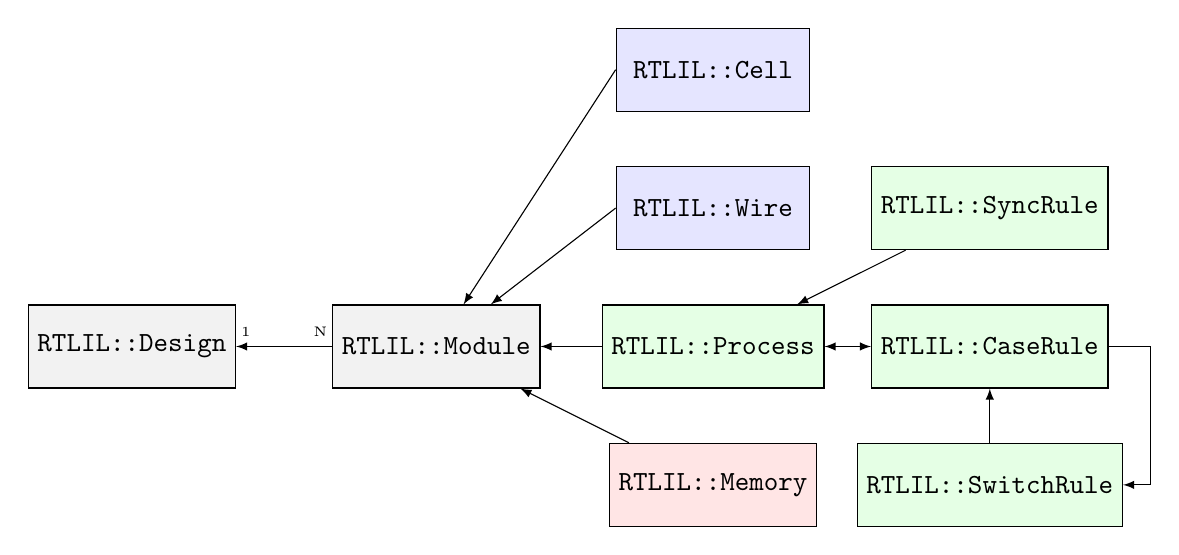
\begin{tikzpicture}
		\tikzstyle{entity} = [draw, fill=gray!10, rectangle, minimum height=3em, minimum width=7em, node distance=5em, font={\ttfamily}]
		\node[entity] (design) {RTLIL::Design};
		\node[entity] (module) [right of=design, node distance=11em] {RTLIL::Module} edge [-latex] node[above] {\tiny 1 \hskip3em N} (design);

		\node[entity] (process) [fill=green!10, right of=module, node distance=10em] {RTLIL::Process} (process.west) edge [-latex] (module);
		\node[entity] (memory) [fill=red!10, below of=process] {RTLIL::Memory} edge [-latex] (module);
		\node[entity] (wire) [fill=blue!10, above of=process] {RTLIL::Wire} (wire.west) edge [-latex] (module);
		\node[entity] (cell) [fill=blue!10, above of=wire] {RTLIL::Cell} (cell.west) edge [-latex] (module);

		\node[entity] (case) [fill=green!10, right of=process, node distance=10em] {RTLIL::CaseRule} edge [latex-latex] (process);
		\node[entity] (sync) [fill=green!10, above of=case] {RTLIL::SyncRule} edge [-latex] (process);
		\node[entity] (switch) [fill=green!10, below of=case] {RTLIL::SwitchRule} edge [-latex] (case);
		\draw[latex-] (switch.east) -- ++(1em,0) |- (case.east);
	\end{tikzpicture}
	\caption{Simplified RTLIL Entity-Relationship Diagram}
	\label{fig:Overview_RTLIL}
\end{figure}

There is only one active RTLIL::Design object that is used by all frontends,
passes and backends called by the user, e.g.~using a synthesis script. The RTLIL::Design then contains
zero to many RTLIL::Module objects. This corresponds to modules in Verilog or entities in VHDL. Each
module in turn contains objects from three different categories:

\begin{itemize}
\item RTLIL::Cell and RTLIL::Wire objects represent classical netlist data.
\item RTLIL::Process objects represent the decision trees (if-then-else statements, etc.) and synchronization
declarations (clock signals and sensitivity) from Verilog {\tt always} and VHDL {\tt process} blocks.
\item RTLIL::Memory objects represent addressable memories (arrays).
\end{itemize}

\begin{sloppypar}
Usually the output of the synthesis procedure is a netlist, i.e. all
RTLIL::Process and RTLIL::Memory objects must be replaced by RTLIL::Cell and
RTLIL::Wire objects by synthesis passes.
\end{sloppypar}

All features of the HDL that cannot be mapped directly to these RTLIL classes must be
transformed to an RTLIL-compatible representation by the HDL frontend. This includes
Verilog-features such as generate-blocks, loops and parameters.

The following sections contain a more detailed description of the different
parts of RTLIL and rationale behind some of the design decisions.

\subsection{RTLIL Identifiers}

All identifiers in RTLIL (such as module names, port names, signal names, cell
types, etc.) follow the following naming convention: they must either start with
a backslash (\textbackslash) or a dollar sign (\$).

Identifiers starting with a backslash are public visible identifiers. Usually
they originate from one of the HDL input files. For example the signal name ``{\tt \textbackslash sig42}''
is most likely a signal that was declared using the name ``{\tt sig42}'' in an HDL input file.
On the other hand the signal name ``{\tt \$sig42}'' is an auto-generated signal name. The backends
convert all identifiers that start with a dollar sign to identifiers that do not collide with
identifiers that start with a backslash.

This has three advantages:

\begin{itemize}
\item First, it is impossible that an auto-generated identifier collides with
an identifier that was provided by the user.
\item Second, the information about which identifiers were originally
provided by the user is always available which can help guide some optimizations. For example the ``opt\_rmunused''
tries to preserve signals with a user-provided name but doesn't hesitate to delete signals that have
auto-generated names when they just duplicate other signals.
\item Third, the delicate job of finding suitable auto-generated public visible
names is deferred to one central location. Internally auto-generated names that
may hold important information for Yosys developers can be used without
disturbing external tools. For example the Verilog backend assigns names in the form {\tt \_{\it integer}\_}.
\end{itemize}

Whitespace and control characters (any character with an ASCII code 32 or less) are not allowed
in RTLIL identifiers; most frontends and backends cannot support these characters in identifiers.

In order to avoid programming errors, the RTLIL data structures check if all identifiers start
with either a backslash or a dollar sign, and contain no whitespace or control characters.
Violating these rules results in a runtime error.

All RTLIL identifiers are case sensitive.

Some transformations, such as flattening, may have to change identifiers provided by the user
to avoid name collisions. When that happens, attribute ``{\tt hdlname}`` is attached to the object
with the changed identifier. This attribute contains one name (if emitted directly by the frontend,
or is a result of disambiguation) or multiple names separated by spaces (if a result of flattening).
All names specified in the ``{\tt hdlname}`` attribute are public and do not include the leading
``\textbackslash``.

\subsection{RTLIL::Design and RTLIL::Module}

The RTLIL::Design object is basically just a container for RTLIL::Module objects. In addition to
a list of RTLIL::Module objects the RTLIL::Design also keeps a list of {\it selected objects}, i.e.
the objects that passes should operate on. In most cases the whole design is selected and therefore
passes operate on the whole design. But this mechanism can be useful for more complex synthesis jobs
in which only parts of the design should be affected by certain passes.

Besides the objects shown in the ER diagram in Fig.~\ref{fig:Overview_RTLIL} an RTLIL::Module object
contains the following additional properties:

\begin{itemize}
\item The module name
\item A list of attributes
\item A list of connections between wires
\item An optional frontend callback used to derive parametrized variations of the module
\end{itemize}

The attributes can be Verilog attributes imported by the Verilog frontend or attributes assigned
by passes. They can be used to store additional metadata about modules or just mark them to be
used by certain part of the synthesis script but not by others.

Verilog and VHDL both support parametric modules (known as ``generic entities'' in VHDL). The RTLIL
format does not support parametric modules itself. Instead each module contains a callback function
into the AST frontend to generate a parametrized variation of the RTLIL::Module as needed. This
callback then returns the auto-generated name of the parametrized variation of the module. (A hash
over the parameters and the module name is used to prohibit the same parametrized variation from being
generated twice. For modules with only a few parameters, a name directly containing all parameters
is generated instead of a hash string.)

\subsection{RTLIL::Cell and RTLIL::Wire}
\label{sec:rtlil_cell_wire}

A module contains zero to many RTLIL::Cell and RTLIL::Wire objects. Objects of
these types are used to model netlists. Usually the goal of all synthesis efforts is to convert
all modules to a state where the functionality of the module is implemented only by cells
from a given cell library and wires to connect these cells with each other. Note that module
ports are just wires with a special property.

An RTLIL::Wire object has the following properties:

\begin{itemize}
\item The wire name
\item A list of attributes
\item A width (buses are just wires with a width > 1)
\item Bus direction (MSB to LSB or vice versa)
\item Lowest valid bit index (LSB or MSB depending on bus direction)
\item If the wire is a port: port number and direction (input/output/inout)
\end{itemize}

As with modules, the attributes can be Verilog attributes imported by the
Verilog frontend or attributes assigned by passes.

In Yosys, busses (signal vectors) are represented using a single wire object
with a width > 1. So Yosys does not convert signal vectors to individual signals.
This makes some aspects of RTLIL more complex but enables Yosys to be used for
coarse grain synthesis where the cells of the target architecture operate on
entire signal vectors instead of single bit wires.

In Verilog and VHDL, busses may have arbitrary bounds, and LSB can have either
the lowest or the highest bit index. In RTLIL, bit 0 always corresponds to LSB;
however, information from the HDL frontend is preserved so that the bus will be
correctly indexed in error messages, backend output, constraint files, etc.

An RTLIL::Cell object has the following properties:

\begin{itemize}
\item The cell name and type
\item A list of attributes
\item A list of parameters (for parametric cells)
\item Cell ports and the connections of ports to wires and constants
\end{itemize}

The connections of ports to wires are coded by assigning an RTLIL::SigSpec
to each cell port. The RTLIL::SigSpec data type is described in the next section.

\subsection{RTLIL::SigSpec}
\label{sec:rtlil_sigspec}

A ``signal'' is everything that can be applied to a cell port. I.e.

\begin{itemize}
\item Any constant value of arbitrary bit-width \\
\null\hskip1em For example: \lstinline[language=Verilog]{1337, 16'b0000010100111001, 1'b1, 1'bx}
\item All bits of a wire or a selection of bits from a wire \\
\null\hskip1em For example: \lstinline[language=Verilog]{mywire, mywire[24], mywire[15:8]}
\item Concatenations of the above \\
\null\hskip1em For example: \lstinline[language=Verilog]|{16'd1337, mywire[15:8]}|
\end{itemize}

The RTLIL::SigSpec data type is used to represent signals. The RTLIL::Cell
object contains one RTLIL::SigSpec for each cell port.

In addition, connections between wires are represented using a pair of
RTLIL::SigSpec objects. Such pairs are needed in different locations. Therefore
the type name RTLIL::SigSig was defined for such a pair.

\subsection{RTLIL::Process}
\label{sec:rtlil_process}

When a high-level HDL frontend processes behavioural code it splits it up into
data path logic (e.g.~the expression {\tt a + b} is replaced by the output of an
adder that takes {\tt a} and {\tt b} as inputs) and an RTLIL::Process that models
the control logic of the behavioural code. Let's consider a simple example:

\begin{lstlisting}[numbers=left,frame=single,language=Verilog]
module ff_with_en_and_async_reset(clock, reset, enable, d, q);
input clock, reset, enable, d;
output reg q;
always @(posedge clock, posedge reset)
	if (reset)
		q <= 0;
	else if (enable)
		q <= d;
endmodule
\end{lstlisting}

In this example there is no data path and therefore the RTLIL::Module generated by
the frontend only contains a few RTLIL::Wire objects and an RTLIL::Process.
The RTLIL::Process in RTLIL syntax:

\begin{lstlisting}[numbers=left,frame=single,language=rtlil]
process $proc$ff_with_en_and_async_reset.v:4$1
	assign $0\q[0:0] \q
	switch \reset
		case 1'1
			assign $0\q[0:0] 1'0
		case
			switch \enable
				case 1'1
					assign $0\q[0:0] \d
				case
			end
	end
	sync posedge \clock
		update \q $0\q[0:0]
	sync posedge \reset
		update \q $0\q[0:0]
end
\end{lstlisting}

This RTLIL::Process contains two RTLIL::SyncRule objects, two RTLIL::SwitchRule
objects and five RTLIL::CaseRule objects. The wire {\tt \$0\textbackslash{}q[0:0]}
is an automatically created wire that holds the next value of {\tt \textbackslash{}q}. The lines
$2 \dots 12$ describe how {\tt \$0\textbackslash{}q[0:0]} should be calculated. The
lines $13 \dots 16$ describe how the value of {\tt \$0\textbackslash{}q[0:0]} is used
to update {\tt \textbackslash{}q}.

An RTLIL::Process is a container for zero or more RTLIL::SyncRule objects and
exactly one RTLIL::CaseRule object, which is called the {\it root case}.

An RTLIL::SyncRule object contains an (optional) synchronization condition (signal and edge-type), zero or
more assignments (RTLIL::SigSig), and zero or more memory writes (RTLIL::MemWriteAction).
The {\tt always} synchronization condition is used to break combinatorial
loops when a latch should be inferred instead.

An RTLIL::CaseRule is a container for zero or more assignments (RTLIL::SigSig)
and zero or more RTLIL::SwitchRule objects. An RTLIL::SwitchRule objects is a
container for zero or more RTLIL::CaseRule objects.

In the above example the lines $2 \dots 12$ are the root case. Here {\tt \$0\textbackslash{}q[0:0]} is first
assigned the old value {\tt \textbackslash{}q} as default value (line 2). The root case
also contains an RTLIL::SwitchRule object (lines $3 \dots 12$). Such an object is very similar to the C {\tt switch}
statement as it uses a control signal ({\tt \textbackslash{}reset} in this case) to determine
which of its cases should be active. The RTLIL::SwitchRule object then contains one RTLIL::CaseRule
object per case. In this example there is a case\footnote{The
syntax {\tt 1'1} in the RTLIL code specifies a constant with a length of one bit (the first ``1''),
and this bit is a one (the second ``1'').} for {\tt \textbackslash{}reset == 1} that causes
{\tt \$0\textbackslash{}q[0:0]} to be set (lines 4 and 5) and a default case that in turn contains a switch that
sets {\tt \$0\textbackslash{}q[0:0]} to the value of {\tt \textbackslash{}d} if {\tt
\textbackslash{}enable} is active (lines $6 \dots 11$).

A case can specify zero or more compare values that will determine whether it matches. Each of the compare values
must be the exact same width as the control signal. When more than one compare value is specified, the case matches
if any of them matches the control signal; when zero compare values are specified, the case always matches (i.e.
it is the default case).

A switch prioritizes cases from first to last: multiple cases can match, but only the first matched case becomes
active. This normally synthesizes to a priority encoder. The {\tt parallel\_case} attribute allows passes to assume
that no more than one case will match, and {\tt full\_case} attribute allows passes to assume that exactly one
case will match; if these invariants are ever dynamically violated, the behavior is undefined. These attributes
are useful when an invariant invisible to the synthesizer causes the control signal to never take certain
bit patterns.

The lines $13 \dots 16$  then cause {\tt \textbackslash{}q} to be updated whenever there is
a positive clock edge on {\tt \textbackslash{}clock} or {\tt \textbackslash{}reset}.

In order to generate such a representation, the language frontend must be able to handle blocking
and nonblocking assignments correctly. However, the language frontend does not need to identify
the correct type of storage element for the output signal or generate multiplexers for the
decision tree. This is done by passes that work on the RTLIL representation. Therefore it is
relatively easy to substitute these steps with other algorithms that target different target
architectures or perform optimizations or other transformations on the decision trees before
further processing them.

One of the first actions performed on a design in RTLIL representation in most
synthesis scripts is identifying asynchronous resets. This is usually done using the {\tt proc\_arst}
pass. This pass transforms the above example to the following RTLIL::Process:

\begin{lstlisting}[numbers=left,frame=single,language=rtlil]
process $proc$ff_with_en_and_async_reset.v:4$1
	assign $0\q[0:0] \q
	switch \enable
		case 1'1
			assign $0\q[0:0] \d
		case
	end
	sync posedge \clock
		update \q $0\q[0:0]
	sync high \reset
		update \q 1'0
end
\end{lstlisting}

This pass has transformed the outer RTLIL::SwitchRule into a modified RTLIL::SyncRule object
for the {\tt \textbackslash{}reset} signal. Further processing converts the RTLIL::Process
into e.g.~a d-type flip-flop with asynchronous reset and a multiplexer for the enable signal:

\begin{lstlisting}[numbers=left,frame=single,language=rtlil]
cell $adff $procdff$6
	parameter \ARST_POLARITY 1'1
	parameter \ARST_VALUE 1'0
	parameter \CLK_POLARITY 1'1
	parameter \WIDTH 1
	connect \ARST \reset
	connect \CLK \clock
	connect \D $0\q[0:0]
	connect \Q \q
end
cell $mux $procmux$3
	parameter \WIDTH 1
	connect \A \q
	connect \B \d
	connect \S \enable
	connect \Y $0\q[0:0]
end
\end{lstlisting}

Different combinations of passes may yield different results. Note that {\tt \$adff} and {\tt
\$mux} are internal cell types that still need to be mapped to cell types from the
target cell library.

Some passes refuse to operate on modules that still contain RTLIL::Process objects as the
presence of these objects in a module increases the complexity. Therefore the passes to translate
processes to a netlist of cells are usually called early in a synthesis script. The {\tt proc}
pass calls a series of other passes that together perform this conversion in a way that is suitable
for most synthesis tasks.

\subsection{RTLIL::Memory}
\label{sec:rtlil_memory}

For every array (memory) in the HDL code an RTLIL::Memory object is created. A
memory object has the following properties:

\begin{itemize}
\item The memory name
\item A list of attributes
\item The width of an addressable word
\item The size of the memory in number of words
\end{itemize}

All read accesses to the memory are transformed to {\tt \$memrd} cells and all write accesses to
{\tt \$memwr} cells by the language frontend. These cells consist of independent read- and write-ports
to the memory. Memory initialization is transformed to {\tt \$meminit} cells by the language frontend.
The \B{MEMID} parameter on these cells is used to link them together and to the RTLIL::Memory object they belong to.

The rationale behind using separate cells for the individual ports versus
creating a large multiport memory cell right in the language frontend is that
the separate {\tt \$memrd} and {\tt \$memwr} cells can be consolidated using resource sharing.
As resource sharing is a non-trivial optimization problem where different synthesis tasks
can have different requirements it lends itself to do the optimisation in separate passes and merge
the RTLIL::Memory objects and {\tt \$memrd} and {\tt \$memwr} cells to multiport memory blocks after resource sharing is completed.

The {\tt memory} pass performs this conversion and can (depending on the options passed
to it) transform the memories directly to d-type flip-flops and address logic or yield
multiport memory blocks (represented using {\tt \$mem} cells).

See Sec.~\ref{sec:memcells} for details about the memory cell types.

\section{Command Interface and Synthesis Scripts}

Yosys reads and processes commands from synthesis scripts, command line arguments and
an interactive command prompt. Yosys commands consist of a command name and an optional
whitespace separated list of arguments. Commands are terminated using the newline character
or a semicolon ({\tt ;}). Empty lines and lines starting with the hash sign ({\tt \#}) are ignored.
See Sec.~\ref{sec:typusecase} for an example synthesis script.

The command {\tt help} can be used to access the command reference manual.

Most commands can operate not only on the entire design but also specifically on {\it selected}
parts of the design. For example the command {\tt dump} will print all selected objects
in the current design while {\tt dump foobar} will only print the module {\tt foobar}
and {\tt dump *} will print the entire design regardless of the current selection.

The selection mechanism is very powerful. For example the command {\tt dump */t:\$add
\%x:+[A] */w:* \%i} will print all wires that are connected to the \B{A} port of
a {\tt \$add} cell.  Detailed documentation of the select framework can be
found in the command reference for the {\tt select} command.

\section{Source Tree and Build System}

The Yosys source tree is organized into the following top-level directories:

\begin{itemize}

\item {\tt backends/} \\
This directory contains a subdirectory for each of the backend modules.

\item {\tt frontends/} \\
This directory contains a subdirectory for each of the frontend modules.

\item {\tt kernel/} \\
This directory contains all the core functionality of Yosys. This includes the
functions and definitions for working with the RTLIL data structures ({\tt
rtlil.h} and {\tt rtlil.cc}), the main() function ({\tt driver.cc}), the
internal framework for generating log messages ({\tt log.h} and {\tt log.cc}),
the internal framework for registering and calling passes ({\tt register.h} and
{\tt register.cc}), some core commands that are not really passes ({\tt
select.cc}, {\tt show.cc}, \dots) and a couple of other small utility libraries.

\item {\tt passes/} \\
This directory contains a subdirectory for each pass or group of passes. For example as
of this writing the directory {\tt passes/opt/} contains the code for seven
passes: {\tt opt}, {\tt opt\_expr}, {\tt opt\_muxtree}, {\tt opt\_reduce},
{\tt opt\_rmdff}, {\tt opt\_rmunused} and {\tt opt\_merge}.

\item {\tt techlibs/} \\
This directory contains simulation models and standard implementations for the
cells from the internal cell library.

\item {\tt tests/} \\
This directory contains a couple of test cases. Most of the smaller tests are executed
automatically when {\tt make test} is called. The larger tests must be executed
manually. Most of the larger tests require downloading external HDL source code
and/or external tools. The tests range from comparing simulation results of the synthesized
design to the original sources to logic equivalence checking of entire CPU cores.

\end{itemize}

\begin{sloppypar}
The top-level Makefile includes {\tt frontends/*/Makefile.inc}, {\tt passes/*/Makefile.inc}
and {\tt backends/*/Makefile.inc}. So when extending Yosys it is enough to create
a new directory in {\tt frontends/}, {\tt passes/} or {\tt backends/} with your sources
and a {\tt Makefile.inc}. The Yosys kernel automatically detects all commands linked with
Yosys. So it is not needed to add additional commands to a central list of commands.
\end{sloppypar}

Good starting points for reading example source code to learn how to write passes
are {\tt passes/opt/opt\_rmdff.cc} and {\tt passes/opt/opt\_merge.cc}.

See the top-level README file for a quick {\it Getting Started} guide and build
instructions. The Yosys build is based solely on Makefiles.

Users of the Qt Creator IDE can generate a QT Creator project file using {\tt
make qtcreator}. Users of the Eclipse IDE can use the ``Makefile Project with
Existing Code'' project type in the Eclipse ``New Project'' dialog (only
available after the CDT plugin has been installed) to create an Eclipse project
in order to programming extensions to Yosys or just browse the Yosys code base.

